\documentclass{article}

\title{Optimizing fusion gain through a simplified whole-device model}

\usepackage{graphicx}
\usepackage{amsmath}
\usepackage{amssymb}
\usepackage[dvipsnames]{xcolor}
\usepackage{siunitx}
\usepackage[margin=1in]{geometry}
\usepackage{parskip}
\usepackage{circuitikz}
\usepackage{bm}

\usepackage{biblatex}
\addbibresource{references.bib}

\newcommand{\jack}[1]{{\color{ForestGreen} #1}}

\begin{document}
\maketitle

\section{Introduction}

This document describes a proposed modeling problem for the summer school hackathon.
We'll first describe the physical picture and motivation, then the governing equations, and finally
the configuration of software components we'll use to investigate it.

The setting is the on-axis plasma in a Z Pinch device, bounded on one end by a cathode and on the
other by an anode.
As the Z Pinch current ramps up, and the plasma undergoes compression, on-axis current must connect
through a Langmuir sheath at both electrodes.
The dynamics of the current can be modeled as a series RLC circuit--a circuit containing a resistor,
an inductor, and a capacitor.
The RLC circuit equations let us relate the plasma current, which can be observed from the solution
of our plasma kinetic or fluid equations, to the plasma voltage gap; that is, the voltage gap
across the plasma-facing electrodes.

The final piece of the picture is adiabatic compression. To a first approximation, we can assume
that the pinch is compressing adiabatically, which gives scaling relations between the plasma current
and the on-axis bulk plasma quantities, such as number density and temperature.

Putting all of these pieces together, there is a potential optimization problem to be investigated:
what combination of circuit and plasma parameters maximizes a quantity of interest such as time-integrated
neutron yield, or perhaps Q-scientific?
If the circuit model, bulk plasma model, and sheath model can all be implemented in a differentiable
program, then the optimization problem can be tackled with a derivative-based optimizer.

\begin{figure}
    \centering
    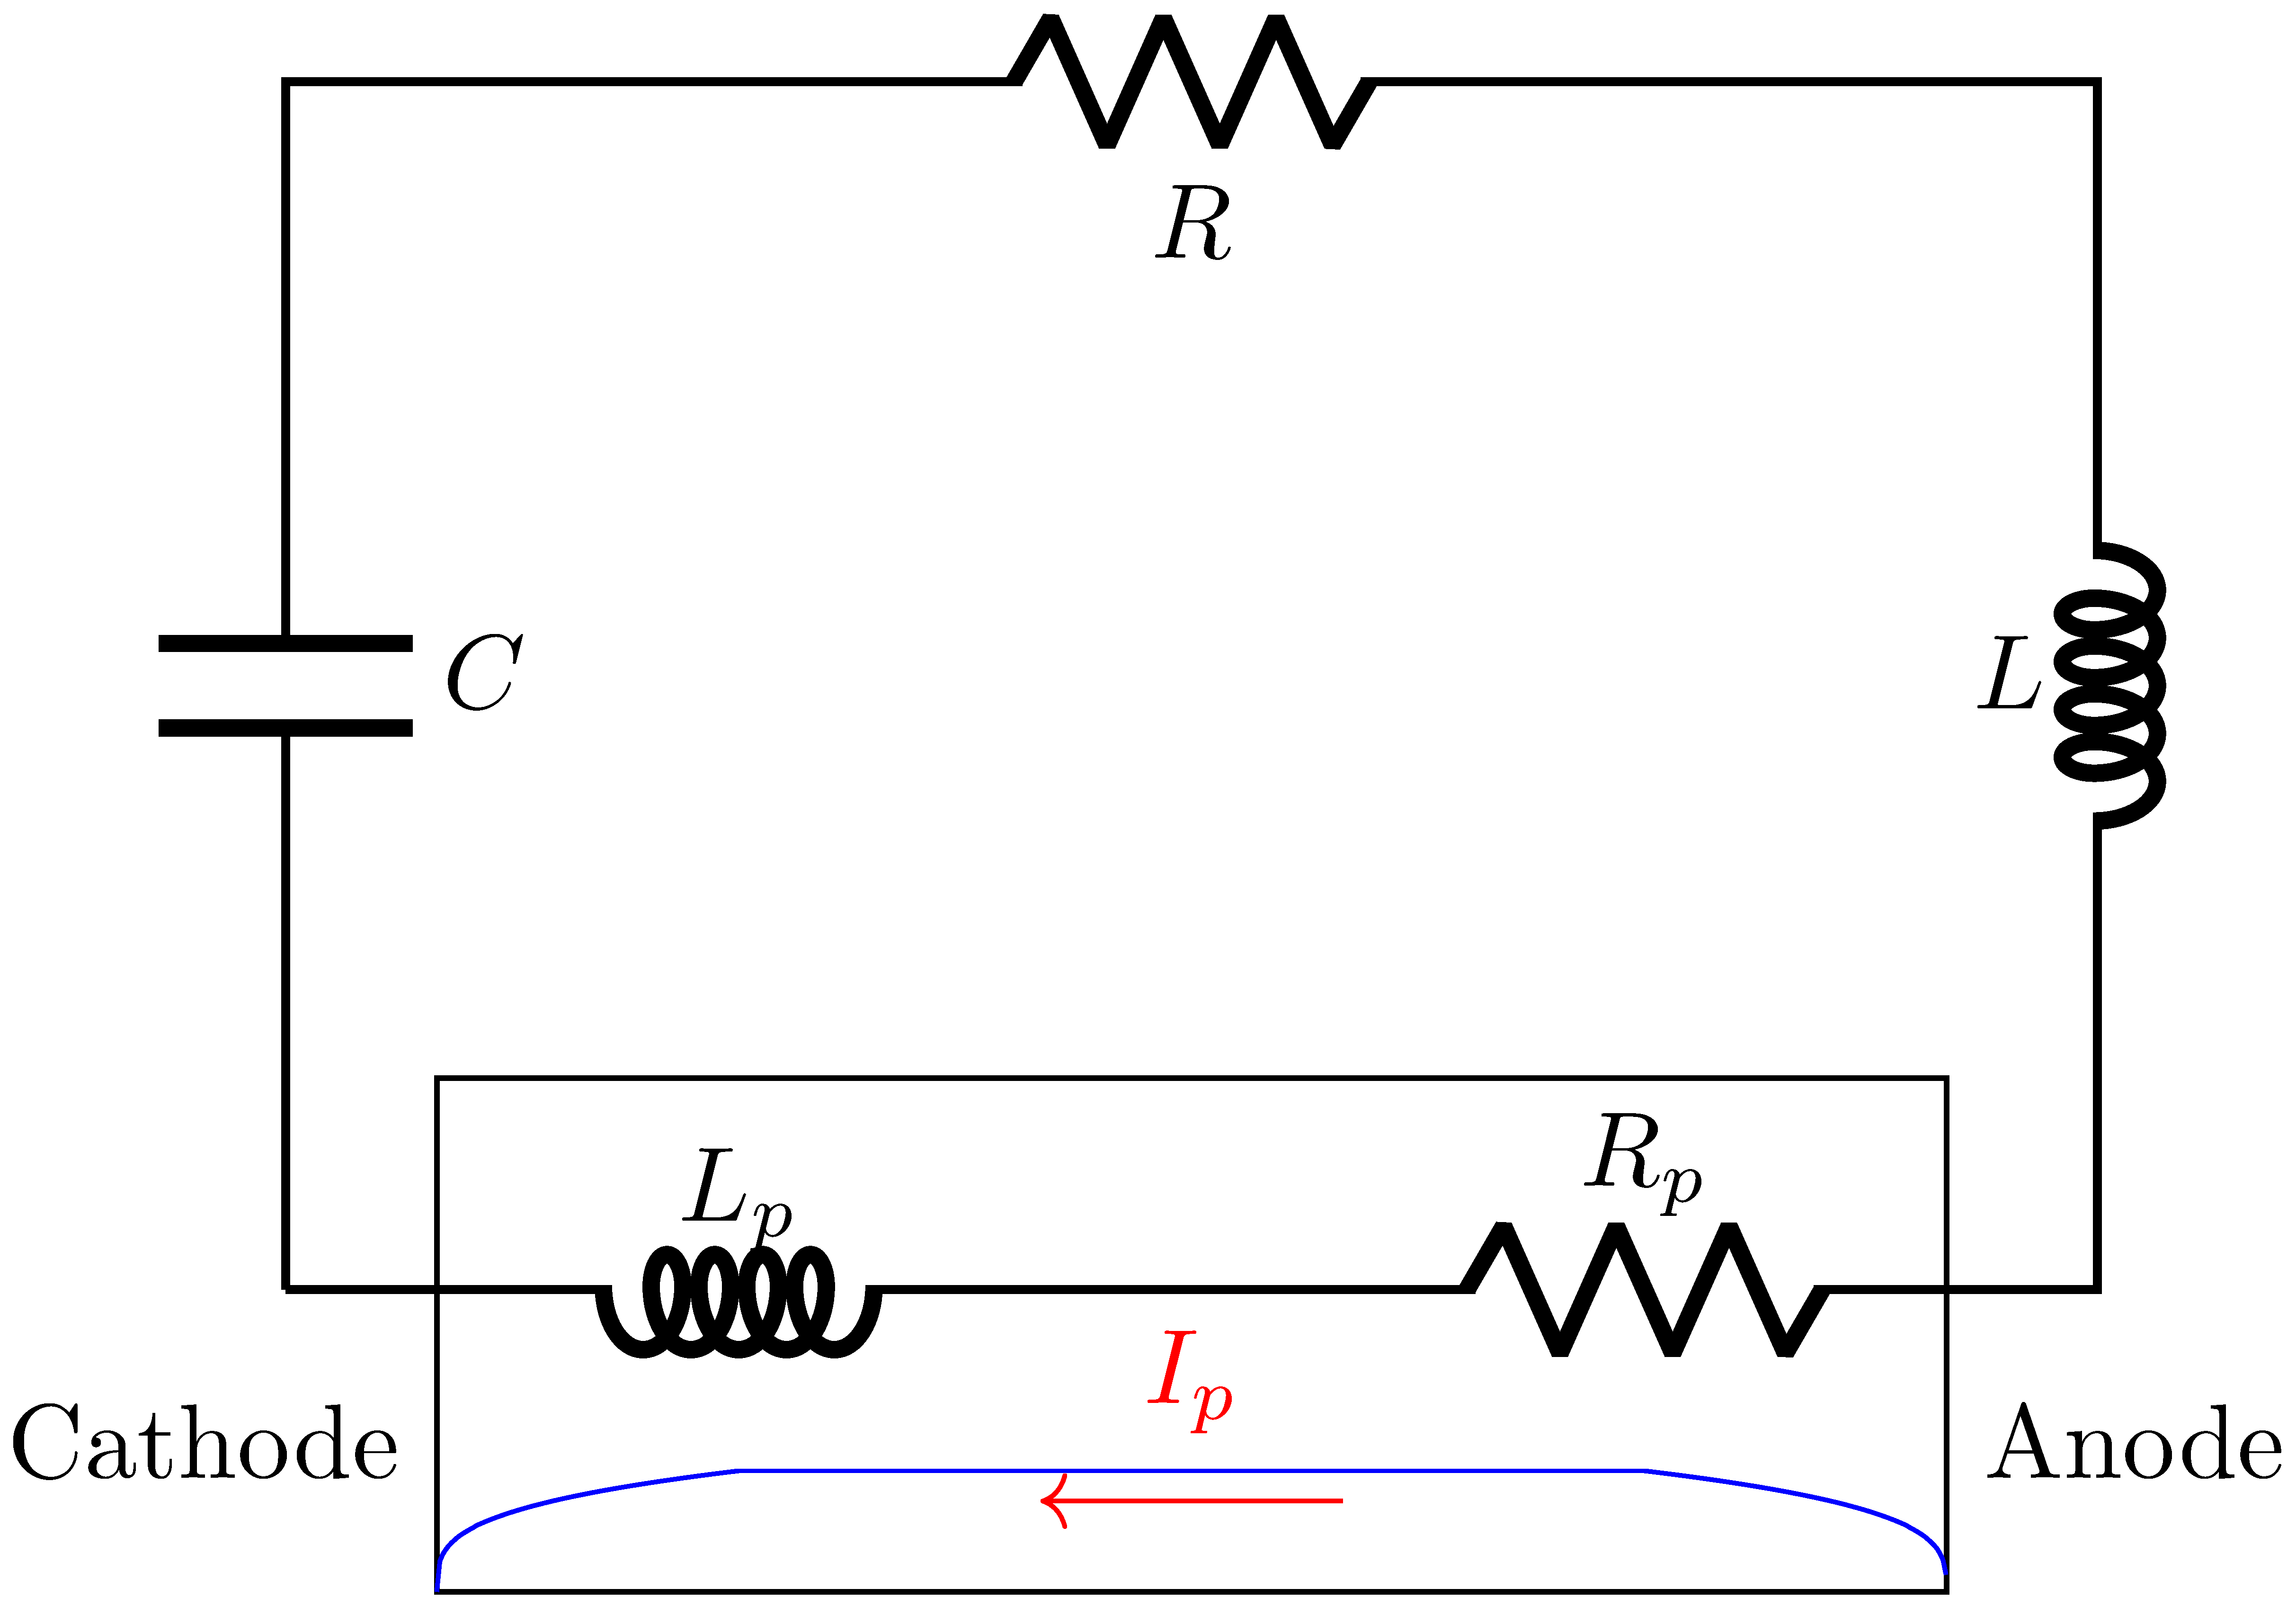
\includegraphics[width=0.6\textwidth]{images/circuit_diagram.pdf}
\end{figure}

\section{Fluid equations for an adiabatically compressing Z pinch}

%The following scaling relations hold for a Z pinch compressing adiabatically from state 1 to state 2 \cite{shumlakShearedFlowStabilizedZPinch2012} with adiabatic index $\gamma = 5/3$.

We begin with the two-fluid continuity equation and the $z$ component of the momentum equation.
These are
\begin{align*}
&\partial_t n_s + \nabla \cdot (n_s \bm{u}_s) = 0 \\
&m_s \partial_t (n_s u_{zs}) + \left[ \nabla \cdot (m_s n_s \bm{u} \otimes \bm{u} + p_s \mathbb{I}) \right]_z = n_s q_s E_z.
\end{align*}
Integrating the continuity equation over the azimuthal direction, and over the radial direction out to the pinch radius $a(t)$,
gives us an equation for the linear density $N(z, t)$:
\begin{align*}
    \partial_t N_s + \partial_z (N_s u_{zs}) = 0,
\end{align*}
where
\begin{align*}
    N(z, t) = \int_0^{2\pi} \int_0^{a(t)} r n \, \mathrm{d} r \, \mathrm{d} \theta.
\end{align*}
is the linear density, defined via an integral out to the pinch radius.
Note that there is no source term, because the radial bounds of integration move with the plasma: $\frac{d a(t)}{dt} = u_r$.
For simplicity we have ignored shear effects and assumed that the axial velocity is uniform within the pinch radius,
so that $u_z = NU_z / N$.

Integrating the $z$ component of momentum over the same bounds, we get
\begin{align*}
    m_s \partial_t (N_s u_{zs}) + \partial_z \left( m_s N_s u_{zs}^2 + P_s \right) = N_s q_s E_z.
\end{align*}
The quantity $P_s$ is the linear density of internal energy, and has units of linear number density times temperature.
We may abuse nomenclature to refer to $P_s$ as the ``linear pressure''.
Here we have assumed that $E_z$ is nearly uniform in the radial direction as well.
This is justified by the very large aspect ratio of the pinch: it is much longer than
it is wide, so a point just off the axis "sees" nearly the same axial variation in electric potential
as a point on the axis.

Instead of an energy equation, we will use an equation of state provided by the scaling relations
satisfied by an adiabatically compressing Z Pinch.
From \cite{shumlakShearedFlowStabilizedZPinch2012}, when compressing from state 1 to state 2, the temperature satisfies
\begin{align*}
\frac{T_2}{T_1} = \left( \frac{I_2}{I_1} \right)^2 \frac{N_1}{N_2},
\end{align*}
where $I$ is the current carried by the pinch.
The linear pressure scales as
\begin{align*}
    \frac{P_2}{P_1} = \frac{T_2}{T_1} \frac{N_2}{N_1} = \left( \frac{I_2}{I_1} \right)^2.
\end{align*}
For our equation of state, we therefore set a reference initial linear pressure, current, and linear density, $P_0, I_0, N_0$, and scale accordingly:
\begin{align*}
    P(N, I) = P_0 \left( \frac{I}{I_0} \right)^{2}
\end{align*}

\section{Poisson solve}

Let $L$ be the length of the whole domain, and let $L_1$, $L_2$ be the locations of the cathode and anode presheath boundaries,
respectively. Our task with the electrode model is to solve for the potential on the subdomains $[0, L_1]$ and $[L_2, L]$.
This is made difficult because $\phi(L_1)$ and $\phi(L_2)$ are floating and cannot be prescribed, so we cannot use Dirichlet
boundary conditions for either subdomain.

Rather, we will derive Robin boundary conditions for both Poisson solves that take into account both the potential drop across
the whole domain and the charge density in the fluid subdomain.

From integrating Gauss's law for $\bm{E}$, we have
\begin{align*}
E_z(z) = \frac{1}{\epsilon_0}\int_0^z \rho_c(z') \, \mathrm{d} z' + E_0
\end{align*}
for some constant $E_0$.
Then the potential at the cathode presheath boundary can be found by integrating
backwards from the anode:
\begin{align*}
    \phi(L_1) &= \phi(L) + \int_{L_1}^L E_z(z) \, \mathrm{d} z \\
              &= \phi(L) + \frac{1}{\epsilon_0} \int_{L_1}^L \int_0^z \rho_c(z') \, \mathrm{d} z' \mathrm{d} z + (L - L_1) E_0
\end{align*}
On the other hand, we have
\begin{align*}
    \phi'(L_1) = -E_z(L_1) = -\frac{1}{\epsilon_0} \int_0^{L_1} \rho_c(z') \, \mathrm{d} z' - E_0
\end{align*}
We can therefore formulate a Robin boundary condition, namely
\begin{align*}
    \phi(L_1) + (L - L_1) \phi'(L_1) = \phi(L) + \frac{1}{\epsilon_0} \left[ -(L-L_1) \int_0^{L_1} \rho_c(z') \, \mathrm{d} z' + \int_{L_1}^L \int_0^z \rho_c(z') \, \mathrm{d} z' \mathrm{d} z \right] 
\end{align*}

On the other side, we have
\begin{align*}
    \phi(L_2) &= \phi(0) + \int_0^{L_2} E_z(z) \, \mathrm{d} z \\
              &= \phi(0) + \frac{1}{\epsilon_0} \int_0^{L_2} \int_0^z \rho_c(z') \, \mathrm{d} z' \mathrm{d} z + L_2 E_0,
\end{align*}
and
\begin{align*}
    \phi'(L_2) = -E_z(L_2) = -\frac{1}{\epsilon_0} \int_0^{L_2} \rho_c(z') \, \mathrm{d} z' - E_0.
\end{align*}
The Robin boundary condition at the anode is therefore
\begin{align*}
    \phi(L_2) + L_2 \phi'(L_2) = \phi(0) + \frac{1}{\epsilon_0} \left[ -L_2 \int_0^{L_2} \rho_c(z') \, \mathrm{d} z' + \int_0^{L_2} \int_0^z \rho_c(z')\,\mathrm{d} z' \mathrm{d} z \right] 
\end{align*}

\section{Fusion gain}
The volumetric number density scales as
\begin{align*}
    \frac{n_2}{n_1} = \left( \frac{I_2}{I_1} \right)^{\frac{2}{(\gamma-1)}} \left( \frac{N_1}{N_2} \right)^{\frac{1}{\gamma-1}}.
\end{align*}

\section{Circuit model}

Series RLC circuit equations for a discharging capacitor.
Let $Q$ be the charge in the capacitor, $C$ the capacitance, $R$ the resistance,
and $L$ the inductance of the circuit.
The circuit current is $I = I_p = \dot{Q}$, the rate of change of the charge.
The voltages of each component are related by
\begin{align}
V_R + V_L + V_C + V_p = 0,
\end{align}
where $V_p$ is the voltage drop across the plasma, and $V_R, V_L, V_C$ are the voltage drops across the resistor, inductor, and capacitor respectively.
From the definition of capacitance we have $V_C = Q/C$. From Ohm's law we have $V_R = IR = \dot{Q} R$, 
and $V_L = \dot{I} L = \ddot{Q} L$.

Solving for the plasma voltage gap, we get
\begin{align*}
V_p = -IR - L \frac{dI}{dt} - C \int_0^t I(\tau) \, \mathrm{d} \tau
\end{align*}

\begin{align*}
    V_{Rp} + V_{Lp} &= -V_R - V_L - V_C \\
    V_{Rp} &= -IR - L \frac{dI}{dt} - L_p \frac{dI}{dt} - C \int_0^t I(\tau) \, \mathrm{d} \tau
\end{align*}

\end{document}
